
\section{Drawing a room onto a cylinder}


The idea here is to imagine a scene taking place in a room. That scene is projected and drawn onto a paper cylinder. This way, a visitor can step inside the cylinder and see the scene around him as if he was actually there. 

This requires two projections to happen to the objects in the scene. Fist we need to project them onto the cylinder. Second we need to roll out the cylinder so that we can actually print the scene on it with a printer or by hand. 

\subsection{Projecting a line in space onto a cylinder}

We want to project the line from $\vec{a} = (10, 10, 1)$ to $\vec{b} = (0, 10, 1)$ onto a cylinder of radius $r=1$. We assume that the visitors eyes will be at the coordinates $\vec{c} = (0, 0, 1.6)$.

\subsubsection{Projecting a point onto the cylinder}

\subsubsection{Projecting a plane onto the cylinder}

So we found out where the two edge points of the line should go onto the cylinder. But what would the line connecting them look like? What we need here is the intersection of the cylinder with the plane  defined by the points $\vec{a}, \vec{b}, \vec{c}$. That plane is expressed as $P = \{ \vec{x} | 0.07y + z = 1.7 \}$.

To find the line we need an expression for $P \intersection C$, that is, a sollution to the system: 

$$ 0.07 y + z = 1.7 $$
$$ x^2 + y^2 = 1 $$

We can factor out $y$, leaving us with $x^2 + (\frac{1.7 - z}{0.07})^2 = 1$

\subsection{Rolling out the cylinder}

We cut the cylinder open along the $z$ axis. That means that for every $z$, we will apply a mapping $(x,y,z) \to (\theta, z)$. One particular mapping really stands out for that purpose - the polar representation of coordinates. Remember that 

$$ cos \theta = \frac{\vec{v}\vec{u}}{|\vec{v}||\vec{u}|}$$

This means that we can achieve our mapping by using $(x,y,z) \to (cos^{-1}x, z)$.


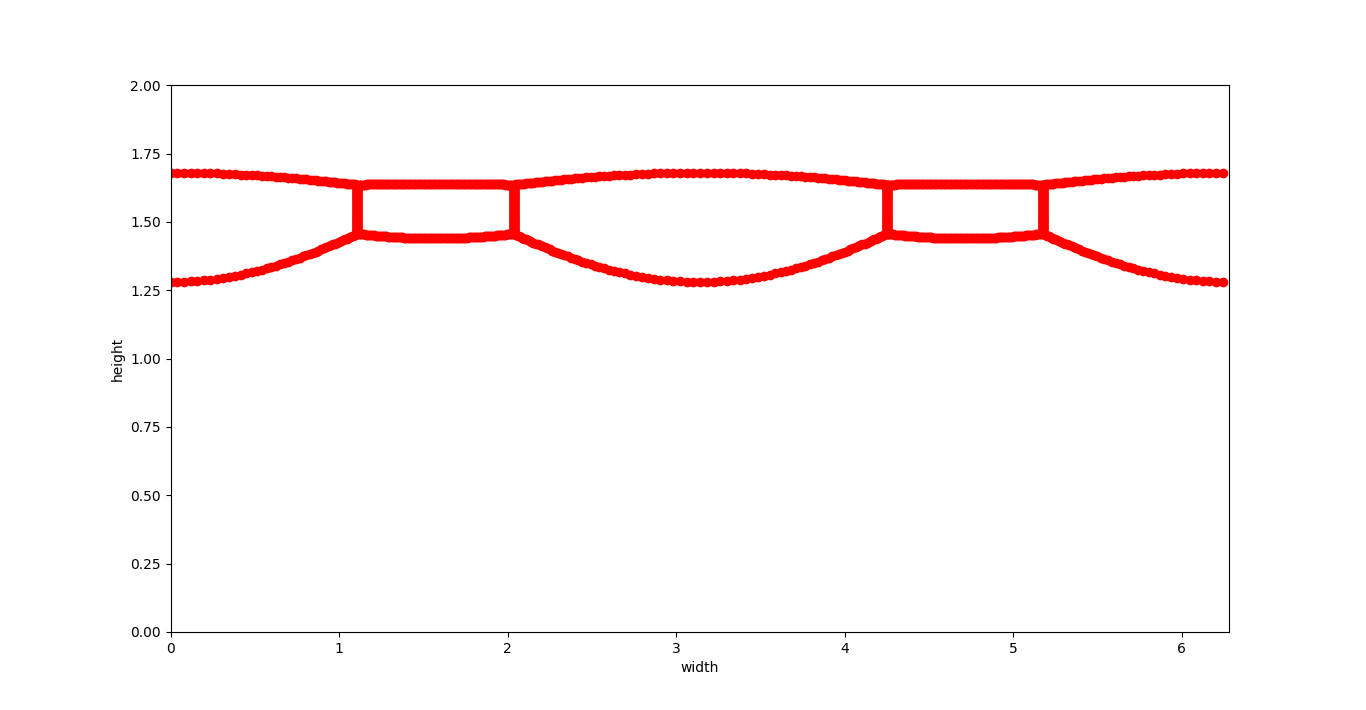
\includegraphics[width=0.8\textwidth]{images/room.png}

\begin{lstlisting}[language=python]
import matplotlib.pyplot as plt
from math import sqrt, pi, acos, atan


def distance(point1, point2):
    return sqrt((point2[0] - point1[0])**2 +
                (point2[1] - point1[1])**2 +
                (point2[2] - point1[2])**2)


def makeLine(point1, point2, num=100):
    line = []
    deltax = float(point2[0] - point1[0])/num
    deltay = float(point2[1] - point1[1])/num
    deltaz = float(point2[2] - point1[2])/num
    for i in range(num):
        x = point1[0] + i*deltax
        y = point1[1] + i*deltay
        z = point1[2] + i*deltaz
        line.append([x, y, z])
    return line


def intersection(point, head, cylinder):
    rc = cylinder.radius
    xp = point[0]
    yp = point[1]
    xh = head[0]
    yh = head[1]
    alpha1 = (xh**2 - xh*xp + yh**2 - yh*yp - sqrt(rc**2*xh**2 - 2*rc**2*xh*xp + rc**2*xp**2 + rc**2*yh**2 - 2*rc**2*yh*yp + rc**2*yp**2 - xh**2*yp**2 + 2*xh*xp*yh*yp - xp**2*yh**2)) / (xh**2 - 2*xh*xp + xp**2 + yh**2 - 2*yh*yp + yp**2)
    alpha2 = (xh**2 - xh*xp + yh**2 - yh*yp + sqrt(rc**2*xh**2 - 2*rc**2*xh*xp + rc**2*xp**2 + rc**2*yh**2 - 2*rc**2*yh*yp + rc**2*yp**2 - xh**2*yp**2 + 2*xh*xp*yh*yp - xp**2*yh**2)) / (xh**2 - 2*xh*xp + xp**2 + yh**2 - 2*yh*yp + yp**2)
    ints1 = [0, 0, 0]
    ints1[0] = head[0] + alpha1*(point[0] - head[0])
    ints1[1] = head[1] + alpha1*(point[1] - head[1])
    ints1[2] = head[2] + alpha1*(point[2] - head[2])
    dist1 = distance(ints1, head)
    ints2 = [0, 0, 0]
    ints2[0] = head[0] + alpha2*(point[0] - head[0])
    ints2[1] = head[1] + alpha2*(point[1] - head[1])
    ints2[2] = head[2] + alpha2*(point[2] - head[2])
    dist2 = distance(ints2, head)
    if dist2 > dist1:
        return ints1
    else:
        return ints2


def toPolar(point):
    pointPolar = [0, 0, 0]
    radius = sqrt(point[0]**2 + point[1]**2)
    #theta = acos(point[0]/radius) * 360.0 / (2*pi)
    theta = atan(point[1]/(point[0] + 0.000001)) * 360.0 / (2*pi)
    if point[0] >= 0 and point[1] >= 0:  # first quad
        theta = theta
    elif point[0] < 0 and point[1] >= 0:  # second quad
        theta = theta + 180
    elif point[0] < 0 and point[1] < 0:  # third quad
        theta = theta + 180
    else:
        theta = theta + 360
    pointPolar[0] = theta
    pointPolar[1] = radius
    pointPolar[2] = point[2]
    return pointPolar


def rollout(point, cylinder):
    pointPolar = toPolar(point)
    newpoint = [0, 0]
    newpoint[0] = 2*pi*cylinder.radius*pointPolar[0]/360
    newpoint[1] = point[2]
    return newpoint


class Cylinder:
    def __init__(self, radius):
        self.radius = radius


cylinder = Cylinder(1)
circumference = 2*pi*cylinder.radius
head = [0, 0, 1.6]
n = 100

# floor
line1 = makeLine([5, 10, 0], [-5, 10, 0], n)
line2 = makeLine([-5, 10, 0], [-5, -10, 0], n)
line3 = makeLine([-5, -10, 0], [5, -10, 0], n)
line4 = makeLine([5, -10, 0], [5, 10, 0], n)

# walls
line5 = makeLine([5, 10, 0], [5, 10, 2], n)
line6 = makeLine([-5, 10, 0], [-5, 10, 2], n)
line7 = makeLine([-5, -10, 0], [-5, -10, 2], n)
line8 = makeLine([5, -10, 0], [5, -10, 2], n)

# ceiling
line9 = makeLine([5, 10, 2], [-5, 10, 2], n)
line10 = makeLine([-5, 10, 2], [-5, -10, 2], n)
line11 = makeLine([-5, -10, 2], [5, -10, 2], n)
line12 = makeLine([5, -10, 2], [5, 10, 2], n)

line = line1 + line2 + line3 + line4 + line5 + line6 + line7 + line8 + line9 + line10 + line11 + line12


out = []
for i in range(len(line)):
    point = line[i]
    ints = intersection(point, head, cylinder)
    projp = rollout(ints, cylinder)
    out.append(projp)
    pointPolar = toPolar(ints)
    #print "mapping [{},{},{}] via ints [{},{},{}] and via polar [{},{},{}] to flat [{},{}]".format(point[0], point[1], point[2], ints[0], ints[1], ints[2], pointPolar[0], pointPolar[1], pointPolar[2], projp[0], projp[1])


xflat = []
yflat = []
for i in range(len(line)):
    xflat.append(out[i][0])
    yflat.append(out[i][1])


plt.plot(xflat, yflat, 'ro')
plt.xlabel('width')
plt.ylabel('height')
plt.axis([0, circumference, 0, 2])
plt.show()
\end{lstlisting}
